\chapter{Application à la prédiction d'entrée manquante}
\graphicspath{{05-Application/}}
Une idée d'application utilisant une architecture de cartes de Kohonen est la prédiction d'entrées. Une architecture de cartes se comporte comme un système dynamique, réagissant aux entrées présentées. Grâce à l'aspect réciproque des connexions, une activité peut être calculée dans une carte ne recevant pas d'entrée externe. Nous montrerons dans ce chapitre que CxSOM permet de prédire une entrée manquante sur une des cartes, de façon dynamique, sans utiliser d'algorithme prédictif supplémentaire. 

\comment{Dire un peu que oui, une carte de Kohonen peut être utilisée pour prédire des entrées, mais que du coup il faut utiliser un algo en plus pour regarder toute la carte. Ici, non, on utilise le même algo dynamique et décentralisé}

\section{Prédiction d'entrées géométrique}

\subsection{Méthodes}
Nous expérimentons d'abord la prédiction sur les données géométriques $X,Y,Z$ utilisées précédemment dans ce rapport. Dans un cercle en trois dimensions, la connaissance de deux dimensions et du modèle géométrique permet d'en prédire la troisième coordonnée.

\begin{figure}
\centering
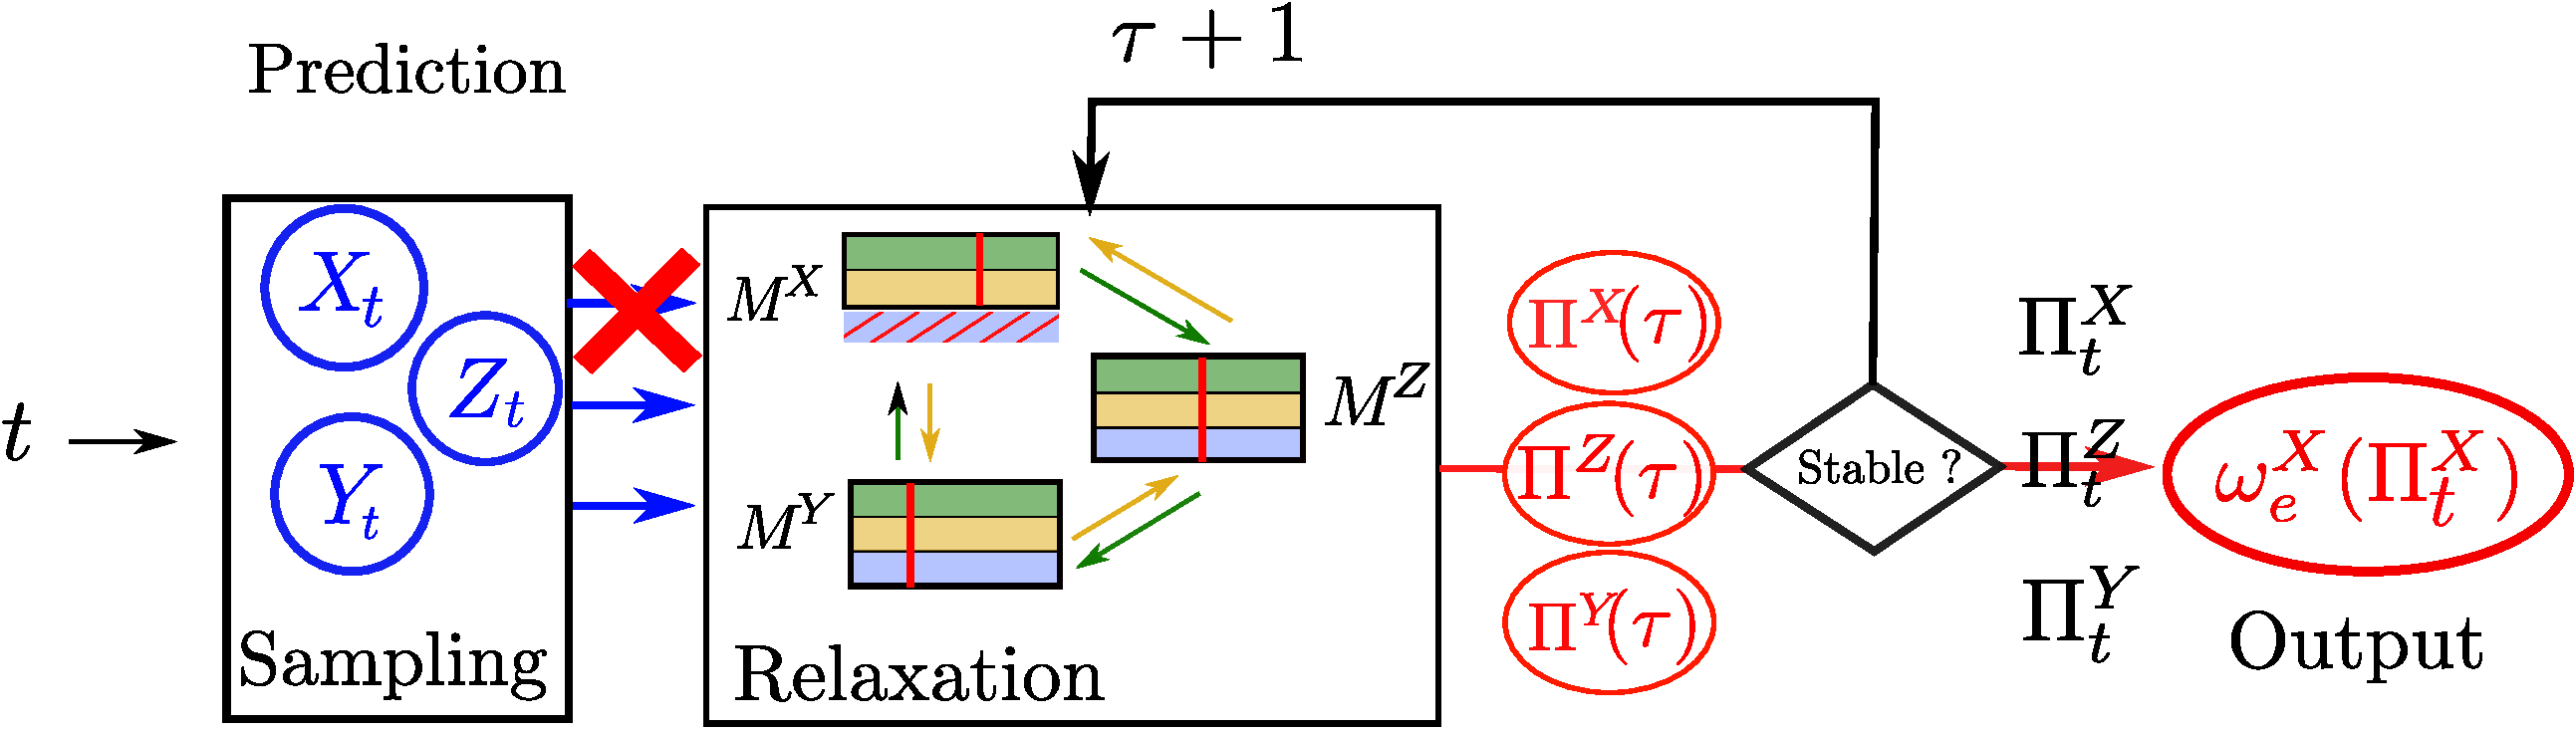
\includegraphics[width=\textwidth]{prediction_setup}
\caption{Description de l'algorithme de prédiction. Il s'agit du même algorithme que pour les tests, sans apprentissage, mais une modalité n'est pas présentée à l'architecture.}
\label{fig:schema}
\end{figure}


\subsection{Résultats}
\section{Commande de drône en vol}